First of all, there is going to be set various criteria for the system, to indicate what general properties is the most crucial. With this, and what have previously been done, the component structure of the system is going to be defined, with the model component and function component. 

\subsubsection{Criteria}

Based on the context of the system, and the system definition, criteria is going to set. This is done to determine which properties is the most important for the system, for the forthcoming development of the system, and limiting the work effort to what is the most crucial. See Table \ref{Criteria}.

\begin{table}[htb]
\centering
\begin{tabular}{|l|c|c|c|c|c|} \hline
	  & \textbf{Very} & \textbf{Important} & \textbf{Less} & \textbf{Irrelevant} & \textbf{Easily Fulfilled} \\ \hline
	\textbf{Usable} &  &  & X &  & \\ \hline
	\textbf{Secure} &  &  &  & X &  \\ \hline
	\textbf{Efficient} &  &  & X &  &  \\ \hline
	\textbf{Correct} &  & X &  &  &  \\ \hline
	\textbf{Reliable} & X &  &  &  &  \\ \hline
	\textbf{Maintainable} &  &  & X &  &  \\ \hline
	\textbf{Testable} & X &  &  &  &  \\ \hline
	\textbf{Flexible} &  & X &  &  &  \\ \hline
	\textbf{Comprehensive} &  &  & X &  &  \\ \hline
	\textbf{Reuseable} &  &  &  & X &  \\ \hline
	\textbf{Portable} &  &  &  & X &  \\ \hline
	\textbf{Interoperable} &  & X &  &  &  \\ \hline
\end{tabular}
\caption{Criteria for the system}
\label{Criteria}
\end{table}

The properties indicated as very important, is ‘Reliable’ and ‘Testable’. Reliable is the property that the system can perform its functions with precision, and reliably every time. This is important because the system is a recommendations system, which requires various algorithms to compare media and users, to generate these recommendations. This functionality should therefore work correctly. Testable is the property that makes it possible for the system to be tested, and ensuring that the systems runs as intended. This is crucial because, with time, the algorithm is most likely going to require various tweaks, and additions, to enhance the performance of the algorithm.

The other three important properties, correct, flexible, and interoperable, is also significant. Correct as an extension to the reliable property, again signifying that it is crucial the algorithm works as intended. Flexible, for the same reasons mentioned above, which is to make it possible to tweak to algorithm and the system to enhance performance. Interoperable, since the system is dependent on external sources to feed it new media data, so the system is up to date with newly released media content.

\subsubsection{Components}

Components is the parts which makes the system, and in this section, these sections is going to be defined, connected, and represented in a diagram. The components for this system is divided into four parts: User interface, functions, model, and external sources or servers. See Figure \ref{Components}.

\begin{figure}[htb]
\centering
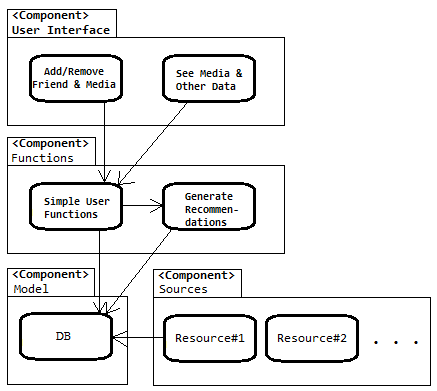
\includegraphics[width=0.7\textwidth]{Images/Components.png}
\caption{The components of the system, divided in layers}
\label{Components}
\end{figure}

The user interface component contains the components which makes it possible for the user using the system, to get access and view data in the system. It has its add and remove component, for both media and friends, and its see component, which retrieves data from system, making it viewable for the user.

Both of these is connected to a component in the function components, which here is called ‘Simple user functions’. This component contains the procedures that retrieves data from the model, and updates the model with data received from the user interface. This component is also connected to another component in the functions layer, called ‘Generate Recommendations’. As previously explained, this procedure is indirectly connected to the user, activated through certain actions performed by the user, or by interval. Actions like the user logging into their account, or changing their preferences.
Both of these components is connected to the model, which all concrete data regarding the users, all the media, and various other notable classes and objects. Right now it is represented by a component called DB, but will be updated to the forthcoming model component.

Using a server pattern, the last part of this component architecture is represented: External sources or servers. These are external servers, which has previously been described, and works together with the update media collections function. It is also through this function that these external sources is connected to the model of the component architecture.